\documentclass[twoside,colorback,accentcolor=tud4c,11pt]{tudreport}

\usepackage{ngerman}
\usepackage[utf8]{inputenc} 
\usepackage[T1]{fontenc}
\usepackage{cancel}
\usepackage{mathtools}
\usepackage{float}
\usepackage{hyperref}
\usepackage{isotope}
\usepackage[deletedmarkup=xout]{changes}
\usepackage{cancel}
\usepackage{gensymb}
\usepackage{siunitx}

\title{VERSUCH 5.4: Tieftemperatur Messung an Suprafluidem Helium }

\subtitle{
\begin{tabular}{p{4cm}ll} 
 Name & Dominik Pfeiffer   &   Jonas Fischer\\
 Matrikelnummer & 2913632  & 2240758 \\
 E-mail& \textaccent{dominik@diepfeiffers.de} & \textaccent{jonas.fischer.42@gmail.com}\\
 \\Versuchsbetreuung & • \\
 Durchführung& 29.05.2017 \\
 Abgabetermin& 19.06.2017
 \end{tabular}}
\institution{Institut für Festkörperphysik}
\sponsor{Wir erklären hiermit, dass die vorliegende Arbeit eigenständig, ohne fremde Hilfe und mit der angegebenen Literatur erarbeitet wurde. Alle Passagen aus Literatur und Internet sind als solche gekennzeichnet. Diese Arbeit liegt weder in gleicher noch ähnlicher Weise einer Prüfungskommission vor.\\\\ 
\begin{tabular}{lp{2em}lp{2em}l}
 \hspace{4cm}   && \hspace{4cm}  && \hspace{4cm}
 \\\cline{1-1}\cline{3-3}\cline{5-5}
    Darmstadt, den \today && Dominik Pfeiffer && Jonas Fischer 
\end{tabular}  
 }   
\begin{document}

\maketitle 

\tableofcontents

\chapter{Ziel des Versuchs}
•
\chapter{Physikalische Grundlagen}
Im folgenden sollen die physikalischen Grundlagen des Versuchs erläutert werden.
\section{Kühlverfahren zum Erreichen tiefer Temperaturen}
Um tiefe Temperaturen - wie in diesem Versuch von wenigen Kelvin - zu erreichen müssen oft mehrere Kühlverfahren angewendet werden. In unserem Versuch wird mit der Verdampfungskühlung (\ref{subsubsec:Verd}) gearbeitet.
\subsubsection{Verflüssigung}
Zur Kühlung der meisten Gase kann der Joule-Thompson Effekt verwendet werden. Ab der Inversionstemperatur kühlen reale Gase bei einer Druckminderung ab. Bei den meisten Gasen liegt diese über Raumtemperatur, nicht jedoch bei Helium, sodass dieses vorgekühlt werden muss.
\subsubsection{Verdampfungskühlung}\label{subsubsec:Verd}
Bei der Verdampfung wird der Flüssigkeit Wärme entzogen. Pumpt man die verdampften Moleküle ab, so liegt der Gasdruck unter dem Dampfdruck und um wieder ein Gleichgewicht herzustellen verdampft mehr Flüssigkeit. Dadurch sinkt die Temperatur entlang der Dampfdruckkurve. Mit dieser Methode erreicht man Temperaturen bis 1 K.
\subsubsection{Adiabatische Entmagnetisierung}
Die Spins der Elektronen oder der Kerne werden in einem Magnetfeld ausgerichtet. Dadurch sinkt die Entropie und die Wärme wird an ein Wärmebad abgegeben. Fährt man nun das Magnetfeld langsam herunter, so bleibt die Entropie erhalten und die Temperatur sinkt. Hiermit können Temperaturen im Milli- und im Falle der Kernspinentmagnetisierung sogar Mikrokelvinbereich erreicht werden.
\subsubsection{\isotope[3]{He}-\isotope[4]{He} Entmischungskühlung}
Ab 0,86 K tritt eine Entmischung der Heliumisotope auf. Dabei entsteht eine suprafluide \isotope[4]{He}-Phase und eine \isotope[3]{He}-Phase. Da sich das \isotope[3]{He} reibungslos im \isotope[4]{He} bewegen kann gleicht das Gleichgewicht einer Verdampfung und es kann mit dem selben Prinzip wie bei der Verdampfungskühlung gearbeitet werden.
\section{Thermometrie bei tiefen Temperaturen}
Bei der Messung von Temperaturen benutzt man ein Gerät dessen Sensor im Gleichgewicht mit dem zu Messenden ist. Dabei können primäre oder Sekundäre Thermometer verwendet werden.
\subsection{Primäre Thermometer}
Bei primären Thermometern ist der Zusammenhang zwischen Messgröße und Temperatur so gut bekannt, dass direkt auf die Temperatur geschlossen werden kann. So ist etwa der Siedepunkt von Wasser bei Normaldruck 100 \degree C, oder die Dampfdruckkurve von \isotope[4]{He} zwischen 0,65 K und 5 K genau bekannt. Will man jedoch größere Temperaturbereiche messen, so benutzt man sekundäre Thermometer.
\subsection{Sekundäre Thermometer}
Bei sekundären Thermometern ist der Zusammenhang zwischen Messgröße und nicht so genau bekannt wie bei primären, sie können jedoch an diesen geeicht werden. Beispiele dafür sind etwa die Ausdehnung von Quecksilber an alten Thermometern oder die Suszeptibilität, die über das Curie-Gesetz (\ref{sec:curie}) $ {\chi=C/T} $ (\ref{eq:curie}) mit der Temperatur verknüpft ist.
\section{Curie-/Curie-Weiss-Gesetz}\label{sec:curie}
Das Curie-Gesetz (\ref{eq:curie}) beschreibt den Zusammenhang der Suszeptibilität mit der Temperatur für einen idealen Paramagneten mit Wechselwirkungsfreien magnetischen Momenten. Berücksichtigt man die Wechselwirkung der magnetischen Momente so kommt man auf das Curie-Weiss-Gesetz:
\begin{align}\label{eq:weiss}
\chi=\frac{C}{T-\theta}
\end{align}
mit der Curie-Konstanten $C$ und der Curie-Temperatur $\theta$.
\subsection{Herleitung des Curie-Gesetztes}
Für ein Atom mit dem Gesamtdrehmoment $\vec{J}$ im äußeren Feld $\vec{B}$ schreibt sich die potentielle Energie als
\begin{equation}
V=\mu_{b} g_{J}\vec{J}\cdot\vec{B}
\end{equation}
dabei gilt $\vec{J}\cdot\vec{B} =m_{z}B_{z}$ mit $m_{z}\in\left[-J,J\right]$. Aus der Boltzmann-Statistik erhält man die Zustandssumme der J+1 möglichen Energiezustände als
\begin{equation}
Z=\sum_{m_{J}=-J}^{J} e^{-m_{z}\cdot\frac{\mu_{b}g_{J}B_{z}}{k_{B}T}}=\sum_{m_{J}=-J}^{J} e^{-m_{z}\cdot\frac{\xi}{J}}\,mit\, \xi = \frac{\mu_{b}g_{J}B_{z}\cdot J}{k_{B}T}.
\end{equation}
Daraus folgt die Darstellung der Zustandssumme über die Hyperbelfunktion sinh zu
\begin{equation}
Z=\frac{\sinh\left(\frac{2J+1}{2J}\cdot\xi\right)}{\sinh\left(\frac{\xi}{2J}\right)}.
\end{equation}
Mit der freien Energie $F=U-TS=-Nk_{B}T\ln(Z)$ ergibt sich für die Magnetisierung M eines idealen Paramagneten folgender Zusammenhang:
\begin{equation}
M=-\frac{1}{V}\frac{\partial F}{\partial B}=-\frac{1}{V}\frac{\partial F}{\partial Z}\frac{\partial Z}{\partial \xi}\frac{\partial \xi}{\partial B}
\end{equation}
und mit den partiellen Ableitungen
\begin{align}
\frac{\partial F}{\partial Z}=&\frac{-Nk_{B}T}{Z}=-Nk_{B}T\cdot\frac{\sinh\left(\frac{\xi}{2J}\right)}{\sinh\left(\frac{2J+1}{2J}\cdot\xi\right)}\\
\frac{\partial Z}{\partial \xi}=&\frac{(2J+1)\sinh\left(\frac{\xi}{2J}\right)\cosh\left(\frac{2J+1}{2J}\cdot\xi\right)-\cosh\left(\frac{\xi}{2J}\right)\sinh\left(\frac{2J+1}{2J}\cdot\xi\right)}{2J\cdot\sinh^2\left(\frac{\xi}{2J}\right)}\\
\frac{\partial \xi}{\partial B}=&\frac{\mu_{b}g_{J}\cdot J}{k_{B}T}
\end{align}
folgt damit für M
\begin{align}
M=&\frac{1}{V}\cdot\frac{\mu_{b}g_{J}\cdot J}{\cancel{ k_{B}T}}\cdot N \cancel{k_{B}T}\cdot\frac{\cancel{\sinh\left(\frac{\xi}{2J}\right)}}{\sinh\left(\frac{2J+1}{2J}\cdot\xi\right)}\cdot\frac{(2J+1)\sinh\left(\frac{\xi}{2J}\right)\cosh\left(\frac{2J+1}{2J}\cdot\xi\right)-\cosh\left(\frac{\xi}{2J}\right)\sinh\left(\frac{2J+1}{2J}\cdot\xi\right)}{2J\cdot\sinh^{\cancel{2}}\left(\frac{\xi}{2J}\right)}\\
=&\frac{N\mu_{b}g_{J}\cdot J}{V}\left[\frac{2J+1}{2J}\cdot\coth\left(\frac{2J+1}{2J}\xi\right)-\frac{1}{2J}\cdot\coth\left(\frac{\xi}{2J}\right)\right]
\end{align}
wobei der Teil in de eckigen Klammern der Brillouin-Funktion $B_{J}(x)$ entspricht. Verwendet man nun die Reihendarstellung $\coth (x)=\frac{1}{x}+\frac{x}{3}+O(x^3)$ für kleine x, was dem Grenzwert $\lim_{\xi\to0}\xi=\lim_{B_{z}\to 0}\xi (B_{z})$ entspricht, so erhält man aus der obigen Darstellung
\begin{align}
M=&\frac{N\mu_{b}g_{J}\cdot \cancel{J}}{V}\cdot\frac{J+1}{\cancel{J}}\frac{\xi}{3}\\
=&\frac{N\mu_{B}g_{J}}{V}\frac{J+1}{3}\frac{\mu_{B}g_{J}B_{z}J}{k_{B}T}\\
=&\frac{N\left(\mu_{B}g_{J}\right)^2B_{z}}{3Vk_{B}}\frac{J(J+1)}{T}.
\end{align}
Die Grenzwertbildung ist gerechtfertigt, wenn das Verhältnis von magnetischer Energie zu thermischer Energie klein ist, wofür nur kleine Magnetfelder verwendet werden können. 
Mit der Beziehung $\chi=\mu_{0}\frac{\partial M}{\partial B}$ findet man schließlich
\begin{equation}\label{eq:curie}
\chi=\mu_{0}\frac{\partial M}{\partial B}=\underbrace{\frac{\mu_{0}N\left(\mu_{B}g_{J}\right)^2}{3Vk_{B}}J(J+1)}_{\equiv C}\cdot\frac{1}{T}=\frac{C}{T}
\end{equation}
das bekannte Curie-Gesetz mit der Curie-Konstanten $C=\frac{\mu_{0}N\left(\mu_{B}g_{J}\right)^2}{3Vk_{B}}J(J+1)$.
\section{Eigenschaften von \isotope[3]{He} und \isotope[4]{He}}
Helium-4 wird unterhalb von 2,1768 K suprafluid. Dies bedeutet, dass es eine verschwindende Viskosität aufweist. Misst man die Wärmekapazität so erkennt man, dass diese bei einer bestimmten Temperatur, der $ \lambda $-Temperatur $ T_\lambda $, sehr hohe Werte annimmt. Unterhalb von $T_\lambda$ ist die Flüssigkeit suprafluid. Dieser makroskopische Quanteneffekt kann anschaulich so erklärt werden, dass sich ab dem $ \lambda $-Punkt die \isotope[4]{He} Atome im Grundzustand befinden und sich die Wellenfunktionen ähnlich einem Bose-Einstein-Kondensat überlagern. Dies erklärt auch warum bei \isotope[3]{He} der $\lambda$-Übergang wesentlich tiefer liegt. Denn \isotope[3]{He} sind Fermionen und können daher nicht wie die \isotope[4]{He} Bosonen in den selben Grundzustand kondensieren. Erst ab sehr viel geringeren Temperaturen bilden sie Paare ähnlich den Cooper-Paaren und es kommt auch hier zum $\lambda$-Übergang. 
\begin{table}[H]
\centering
\begin{tabular}{|c|c|c|}
\hline 
 & \isotope[3]{He} & \isotope[4]{He} \\  
\hline 
Siedetemperatur $ T_c $ & 3,19 K & 4,21 K \\
\hline 
$\lambda$-Temperatur $T_{\lambda}$& 0,0025 K & 2,1768 K \\
\hline 
Schmelzdruck bei 0 K & 34,39 bar & 25,36 bar\\ 
\hline 
Spin & $ \frac{1}{2} $ & 0 \\ 
\hline 
\end{tabular} 
\caption{Eigenschaften von \isotope[3]{He} und \isotope[4]{He}.}\label{tab:He}
\end{table}
Bei den in Tabelle \ref{tab:He} aufgeführten Eigenschaften fällt auf, dass Helium einen nicht verschwindenden Schmelzdruck besitzt, was dazu führt, dass Helium keinen Tripelpunkt hat.
\chapter{Versuchsdurchführung und Auswertung}
Im folgenden Abschnitt sind sowohl die Durchführung, als auch dessen Auswertung des Versuches dargestellt.
\section{Heliumsäule}
Da der Ort der Probe im Dewar-Gefäß bei $h_{Probe}=0\,\si{cm}$ angesehen werden kann, der Druck jedoch über der Oberfläche der Heliumsäule gemessen wird, ergibt sich eine Druck und damit eine Temperaturdifferenz zwischen dem Ort der Probe und Ort der Durckmessung. Für den Druck am Probenort gilt:
\begin{equation}
p_{Probe}=p_{Messung}+p_{Probe}=p_{Messung}+\rho_{He,fluid}\cdot h \cdot g
\end{equation}
mit der Dichte für Flüssiges Helium $\rho_{He,fluid}=0,145\,\si{\frac{g}{cm^3}}$. In \ref{ptkorr} sind die Werte des Drucks und der Temperatur sowie deren Differenz zwischen Probenort und Messort aufgelistet.
\begin{table}[H]
\centering
\begin{tabular}{|c|c|c|c|c|c|c|}
\hline 
T in K & h in cm & $p_{Messung}$ in Torr & $p_{Probe}$ in Torr & $T_{Probe}$ in K & $\Delta$p in Torr & $\Delta$T in K\\ 
\hline 
4,2 & 44 & 744 & 748,98 & 4,2066 & 4,69 & 0,0066 \\ 
\hline 
3,4 & 36 & 312 & 315,87 & 3,4098 & 3,84 & 0,0098 \\ 
\hline 
2,9 & 33 & 155 & 158,26 & 2,9145 & 3,52 & 0,0145 \\ 
\hline 
2,2 & 29,5 & 50 & 43,16 & 2,2317 & 3,15 & 0,0317 \\ 
\hline 
2,18 & 28,5 & 38 & 41,04 & 2,2104 & 3,04 & 0,0304 \\ 
\hline 
2,1 & 27,5 & 31 & 33,99 & 2,1344 & 2,93 & 0,0344 \\ 
\hline 
1,7 & 25,4 & 8,5 & 11,17 & 1,7735 & 2,71 & 0,0735 \\ 
\hline 
\end{tabular}
\caption{Werte des gemessenen und des korrigierten Druckes und der Temperatur}\label{ptkorr}
\end{table} 
Da bei dem Aufbau die Sichtfenster der beiden Dewar-Gefäße nicht zu 100\% übereinander lagen, konnte die Höhe auf der Skala nicht sehr exakt abgelesen werden und ein Ablesefehler von $\Delta h=0,5?\,\si{cm}$ ist anzunehmen. Deshalb kommt es zur Anomalie, dass die Temperaturdifferenz für $T=2,18\,\si{K}$ geringer ist als die von $T=2,2\,\si{K}$. Dies dürfte laut Dampfdruckkurve nicht der Fall sein. Des Weiteren gilt für Temperaturen deutlich über dem $\lambda$-Punkt, dass die Temperaturdifferenz verschwindend gering gegenüber dem Temperaturwert und deshalb nicht beachtet werden muss, sowie dass unterhalb des $\lambda$-Punkts jegliche Wärme aufgrund der enorm hohen Wärmeleitfähigkeit des superfluiden Heliums sofort abgeführt wird und deshalb keine Differenz in der Temperatur zustande kommt.
\section{Curie- und Curie-Weiss-Fit}
Wir überprüfen nun, ob die gemessene Suszeptibilität mit dem Curie- bzw. dem Curie-Weiss-Gesetz übereinstimmt und wollen mit den gemessenen Werten dann unser Thermometer kalibrieren. In Abbildung \ref{fig:CW} ist die gemessene Suszeptibilität über die Temperatur aufgetragen. Wir fitten an die Funktionen
\begin{align}
\chi_{\text{C}}&=\chi_0+\frac{C}{T}\\
\chi_{\text{CW}}&=\chi_0+\frac{C}{T-\theta},
\end{align}
da wir das Leersignal berücksichtigen müssen.
\begin{figure}[H]
\centering
   	\begin{minipage}[b]{\textwidth}
   	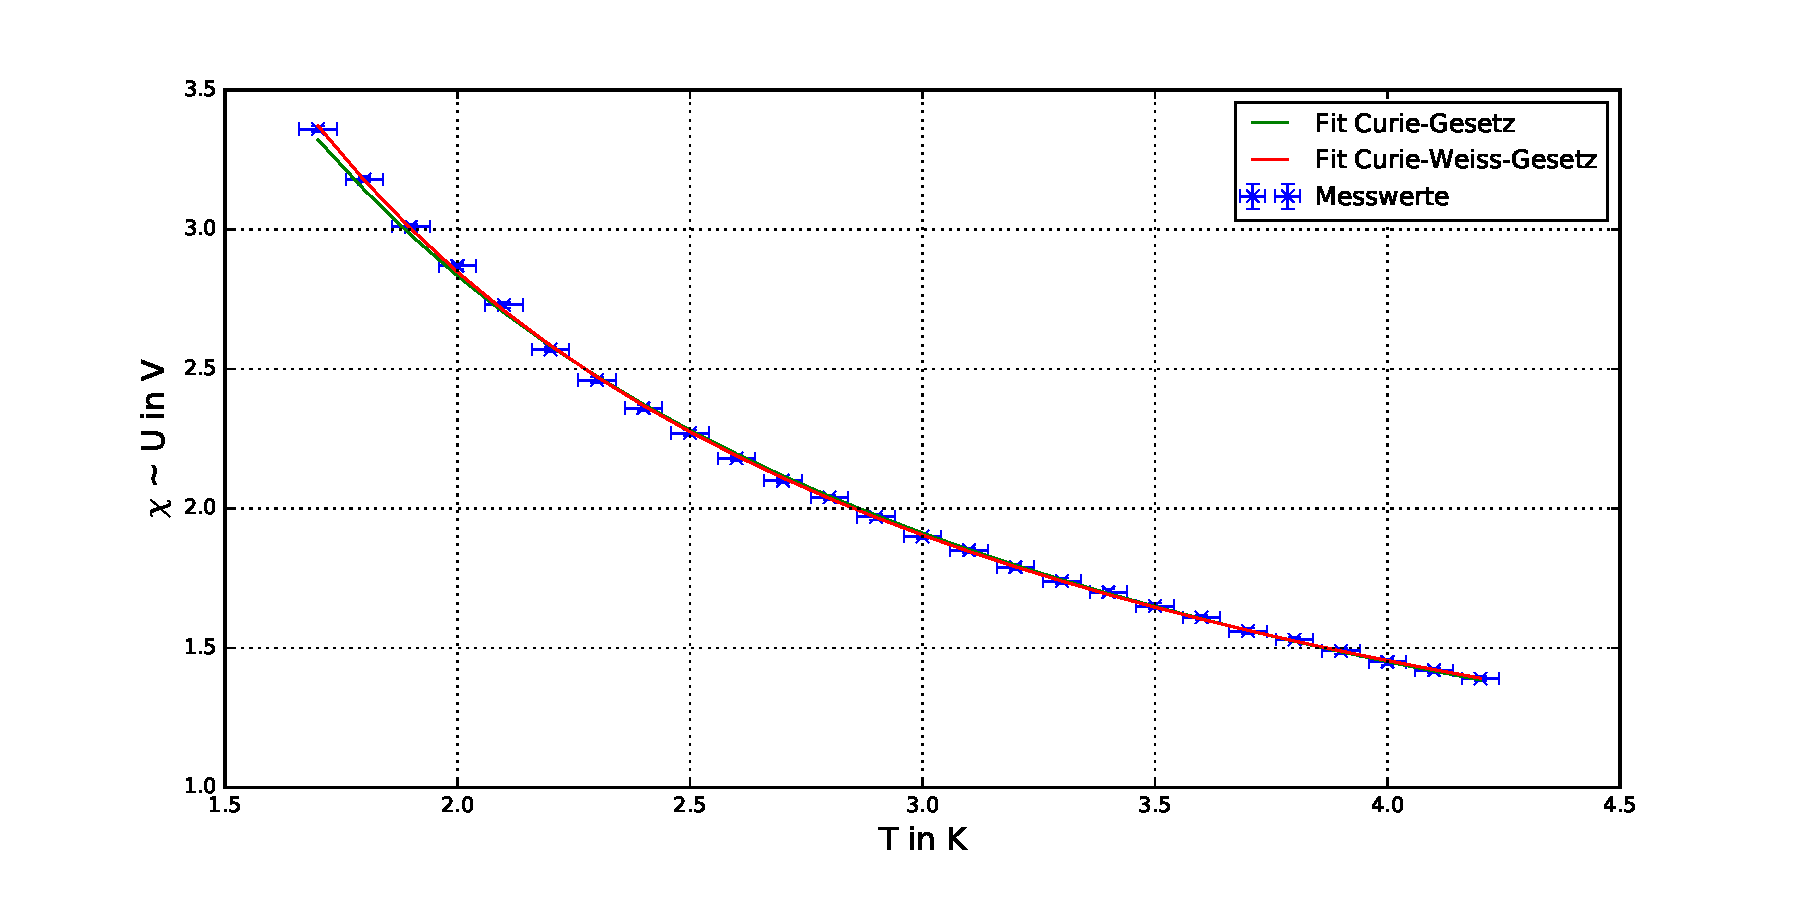
\includegraphics[width=\textwidth]{graphics/chifit.pdf}
   	\caption{Curie- und Curie-Weiss-Fit an die gemessene Suszeptibilität}
  	\label{fig:CW}
   	\end{minipage}
\end{figure}
Man kann erkennen, dass das Curie-Weiss-Gesetz eine etwas bessere Beschreibung der Daten liefert als das Curie-Gesetz. Daher benutzen wir das Curie-Weiss-Gesetz zur Bestimmung der Temperatur in folgender Form:
\begin{align}
\chi_{\text{CW}}(T)=\chi_0+\frac{C}{T-\theta}\sim 0,184+\frac{4,861}{T-0,175}\,[\si{V}]
\end{align}
In Tabelle \ref{tab:fits} sind die Ergebnisse der Fits mit den entsprechenden Ungenauigkeiten aufgetragen.

\begin{table}[H]
\centering
\begin{tabular}{|c|c|c|c|}
\hline 
 & $ \chi_0 $ & $C$ & $\theta$ \\ 
\hline 
$ \chi_{\text{C}} $ & $ 0,069\pm 0,008 $ & $5,531\pm 0,028 $& - \\ 
\hline 
$ \chi_{\text{CW}} $ & $ 0,184\pm 0,020 $ & $  4,861\pm 0,111$ & $  0,175\pm 0,030$ \\ 
\hline 
\end{tabular} 
\caption{Fehler und Parameter der Fits.}\label{tab:fits}
\end{table}
Damit ergibt sich für die Temperatur $T$
\begin{align}
T_{\text{CW}}(\chi)=\frac{C}{\chi-\chi_0}+\theta
\end{align} 
und für den Fehler
\begin{align}
\Delta T_{\text{CW}}(\chi)=\sqrt{\left(\Delta\theta\right)^2+\left(\frac{\Delta C}{\chi-\chi_0}\right)^2+\left(\frac{C\Delta\chi}{(\chi-\chi_0)^2}\right)^2+\left(\frac{C\Delta\chi_0}{(\chi-\chi_0)^2}\right)^2}
\end{align}
Damit ist $ \Delta T $ unseres Thermometers im gemessenen Bereich maximal $ \Delta T_{\text{max}}=0,216\,\si{K} $. Hierfür wurde $ \chi\sim 1\pm 0,01\,\si{V} $ angenommen.
\section{Aufwärmphase}
Nachdem im ersten Teils des Versuches das Heliumbad durch Abpumpen des verdampften Heliums immer weiter bis auf $T=1,7\,\si{K}$ abgekühlt wurde, sollte eine Messreihe während der Aufwärmphase des Heliums aufgenommen werden. Hierfür wurde die Pumpe angestellt und in einem Zeitraum von $t_{Aufwärm}=75\,\si{min}$ in einem Abstand von $\Delta t=5\,\si{min}$ Wertepaare der gemessenen Probenspannung und des Druckes in Torr aufgenommen.
\subsection{pT-Diagramm}
Die aufgenommenen Werte der Probenspannung wurden über die Temperatureichung in Temperaturen umgerechnet das sich so ergebende pT-Diagramm in \ref{pTdia} aufgetragen. Anschließend wurden an die Werte zwei lineare Fits angefertigt.
\begin{figure}[H]
\centering
   	\begin{minipage}[b]{1.0\textwidth}
   	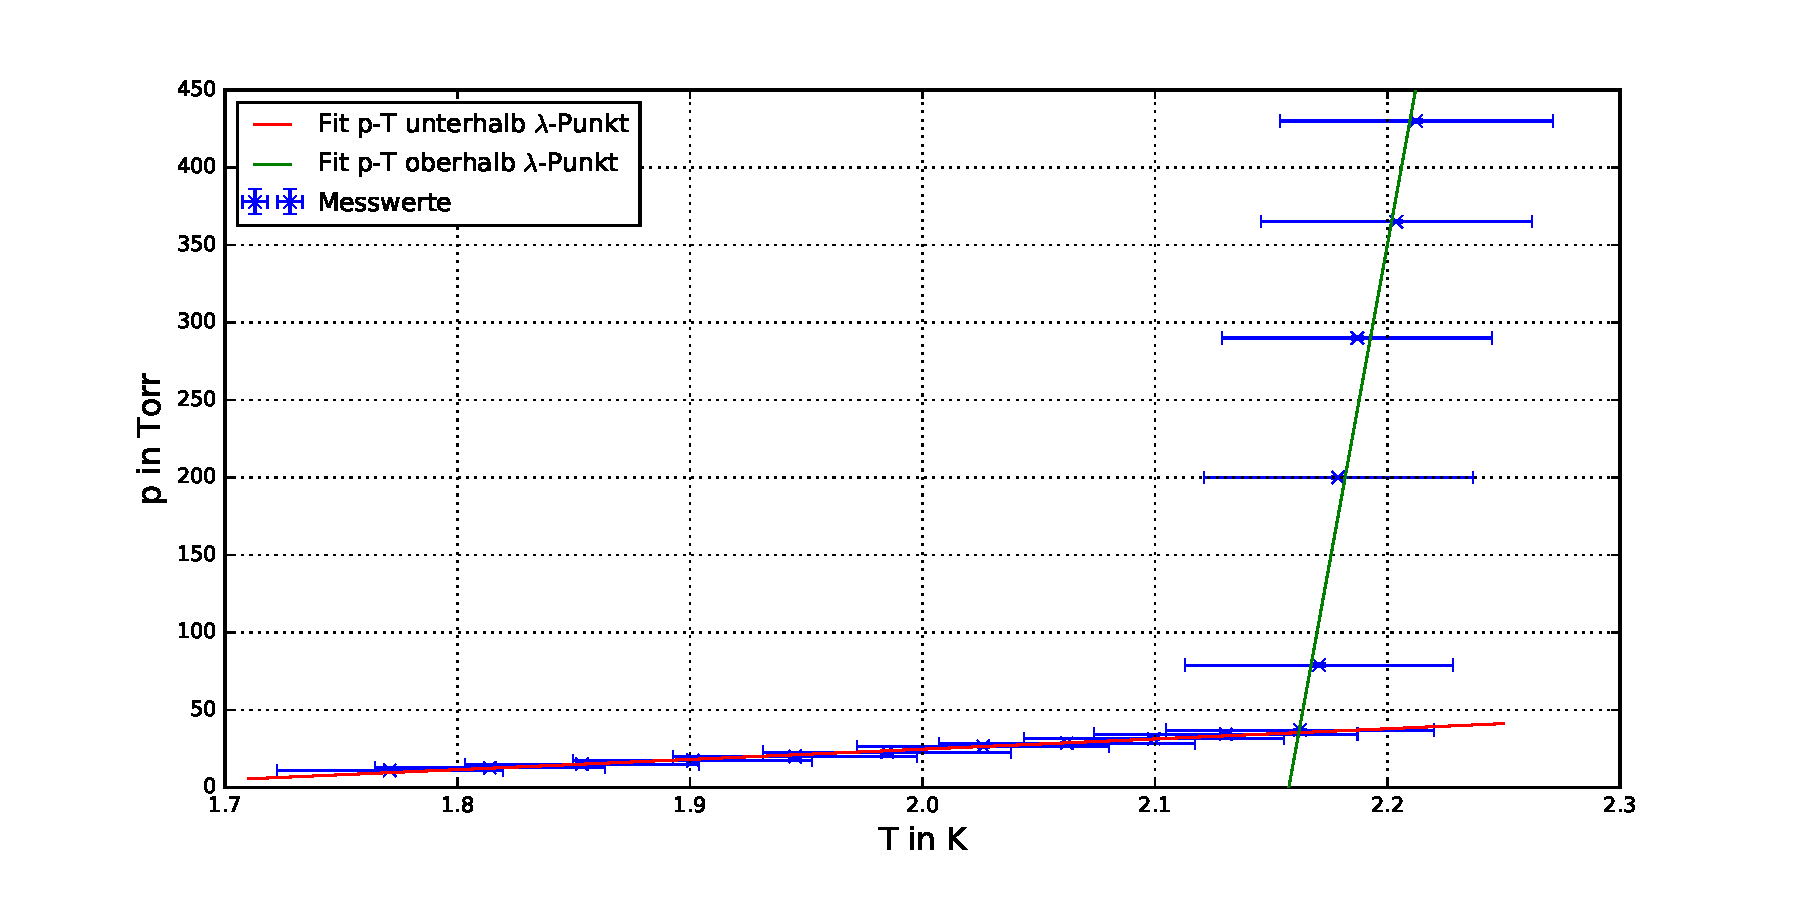
\includegraphics[width=\textwidth]{graphics/pT.pdf}
  	\label{pTdia}
   	\end{minipage}
\caption{pT-Diagramm während der Aufwärmphase mit Ausgleichsgeraden}	
\end{figure}
Für die Fitfunktionen wurden folgende Werte ermittelt:
\begin{align}
m_{u.\lambda}&=65,55\pm 2,39 \,\si{\frac{Torr}{K}}\\
b_{u.\lambda}&=-106,39\pm 4,66\,\si{Torr}\\
m_{o.\lambda}&=8269,48\pm 782,23 \,\si{\frac{Torr}{K}}\\
b_{o.\lambda}&=-17842,11\pm 1709,67\,\si{Torr}
\end{align}
Aus diesen Werten ergibt sich über $T_{\lambda}=\frac{b_{u.\lambda}-b_{o.\lambda}}{m_{o.\lambda}-m_{u.\lambda}}$ die Temperatur des $\lambda$-Punkts zu\\ $T_{\lambda}=2,1619\pm 0,293\,\si{K}$.\\
Im pT-Diagramm macht sich der $\lambda$-Punkt an der Knickstelle bzw. der Schnittstelle der beiden Fitfunktionen bemerkbar. Dies liegt daran, dass Helium am $\lambda$-Punkt eine quasi unendlich hohe Wärmekapazität aufweist, darüber jedoch deutlich geringere Werte annimmt. Der hier bestimmte Temperaturwert  weicht um $0,0149\,\si{K}$ nach unten vom in der Anleitung angegebenen Literaturwert $T_{\lambda}=2,1768\,\si{K}$ ab. Betrachtet man den Fehler der Temperatureichung von $\Delta T=\pm 0,216\,\si{K}$, so liegt der Literaturwert deutlich in der $\sigma$-Umgebung um den errechneten Wert.Die relative Abweichung des errechneten Wertes vom Literaturwert beträgt $\Delta_{rel}=\frac{\Delta T_{\lambda}}{T_{\lambda ,Lit.}}\approx 0,68\%.$ Die Eichung der Temperatur entlang der Helium-Dampfdruckkurve sowie der Curie-Weiss-Fit an die Daten war also hinreichend exakt, um den $\lambda$-Punkt von Helium zu bestimmen.
\chapter{Fazit}	
•
\renewcommand{\bibname}{Literatur}
\begin{thebibliography}{0}
\bibitem {anl} Versuchsanleitung: Thermometrie bei tiefen Temperaturen, Stand 29.05.2017

\end{thebibliography}
\end{document}    
